\documentclass[tikz,border=6pt]{standalone}
\usepackage[utf8]{inputenc}
\usepackage{amsmath}
\usepackage{xcolor}
\usetikzlibrary{arrows.meta,calc,angles,quotes}
\definecolor{azul}{HTML}{1E3A8A}
\definecolor{rojo}{HTML}{DC2626}
\definecolor{verde}{HTML}{16A34A}
\definecolor{gris}{HTML}{64748B}
\definecolor{naranja}{HTML}{F59E0B}
\definecolor{violeta}{HTML}{7C3AED}
\begin{document}
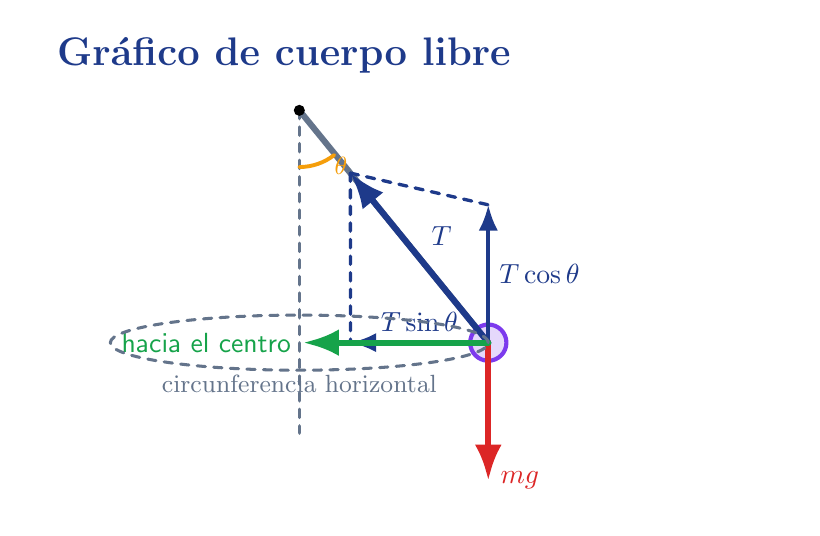
\begin{tikzpicture}[>=Latex, line cap=round, line join=round, font=\sffamily]
  \fill[white] (-4.7,-3.0) rectangle (5.0,3.1);
  \node[azul, font=\bfseries\Large, anchor=west] at (-4.45,2.75) {Gráfico de cuerpo libre};

  \coordinate (P) at (-1.25,2.05);   % punto de suspensión
  \coordinate (B) at (1.15,-0.9);    % masa
  \coordinate (C) at (-1.25,-0.9);   % centro de la circunferencia horizontal

  % Eje vertical y cuerda
  \draw[gris, dashed, line width=1.2pt] (P) -- (-1.25,-2.05);
  \draw[gris, line width=2.2pt] (P) -- (B);
  \fill[black] (P) circle (2pt);
  \draw[violeta, fill=violeta!20, line width=1.5pt] (B) circle (0.23);

  % Ángulo con la vertical
  \draw[naranja, line width=1.4pt] ($(P)+(0,-0.72)$) arc[start angle=-90, end angle=-52, radius=0.72];
  \node[naranja, font=\small] at (-0.72,1.35) {$\theta$};

  % Fuerzas reales
  \draw[->, azul, line width=2.2pt] (B) -- ($(B)!0.73!(P)$) node[midway,above right] {$T$};
  \draw[->, rojo, line width=2.2pt] (B) -- ++(0,-1.75) node[right] {$mg$};

  % Componentes de T
  \coordinate (Ttip) at ($(B)!0.73!(P)$);
  \coordinate (Tvert) at ($(B)+(0,1.75)$);
  \coordinate (Trad) at ($(B)+(-1.75,0)$);
  \draw[azul, dashed, line width=1.2pt] (Ttip) -- (Tvert);
  \draw[azul, dashed, line width=1.2pt] (Ttip) -- (Trad);
  \draw[->, azul, line width=1.4pt] (B) -- (Tvert) node[midway,right] {$T\cos\theta$};
  \draw[->, azul, line width=1.4pt] (B) -- (Trad) node[midway,above] {$T\sin\theta$};

  % Dirección centrípeta
  \draw[->, verde, line width=2.2pt] (B) -- ($(B)+(-2.35,0)$) node[left] {hacia el centro};
  \draw[gris, dashed, line width=1.1pt] (C) ellipse (2.4 and 0.35);
  \node[gris, font=\small] at (-1.25,-1.42) {circunferencia horizontal};
\end{tikzpicture}
\end{document}
